% \iffalse meta-comment
% 
% Copyright (C) 2019 by Alejandro Ochoa <https://ochoalab.github.io/>
%
% This file may be distributed and/or modified under the
% conditions of the LaTeX Project Public License, either
% version 1.3c of this license or (at your option) any later
% version.  The latest version of this license is in:
%
%    http://www.latex-project.org/lppl.txt
%
% and version 1.3c or later is part of all distributions of
% LaTeX version 2006/05/20 or later.
%
% You can obtain the latest version of this package from
%
%    http://github.com/alexviiia/kinshipsymbols
%
% \fi
%
% \iffalse
%<package>\NeedsTeXFormat{LaTeX2e}
%<package>\ProvidesPackage{kinshipsymbols}
%<package>   [2020/03/05 v1.01 Math symbols for statistical genetics models, particularly kinship coefficients, including options like colors and notation simplifications]
%<*driver>
\documentclass{ltxdoc}
\usepackage{kinshipsymbols}
\usepackage{graphicx} % to insert figures into manual
\usepackage{hyperref} % for a link in the manual
\usepackage[capitalize]{cleveref} % to reference figures
\EnableCrossrefs
\CodelineIndex
\RecordChanges
\begin{document}
  \DocInput{kinshipsymbols.dtx}
\end{document}
%</driver>
% \fi
%
% \CheckSum{339}
%
% \CharacterTable
%  {Upper-case    \A\B\C\D\E\F\G\H\I\J\K\L\M\N\O\P\Q\R\S\T\U\V\W\X\Y\Z
%   Lower-case    \a\b\c\d\e\f\g\h\i\j\k\l\m\n\o\p\q\r\s\t\u\v\w\x\y\z
%   Digits        \0\1\2\3\4\5\6\7\8\9
%   Exclamation   \!     Double quote  \"     Hash (number) \#
%   Dollar        \$     Percent       \%     Ampersand     \&
%   Acute accent  \'     Left paren    \(     Right paren   \)
%   Asterisk      \*     Plus          \+     Comma         \,
%   Minus         \-     Point         \.     Solidus       \/
%   Colon         \:     Semicolon     \;     Less than     \<
%   Equals        \=     Greater than  \>     Question mark \?
%   Commercial at \@     Left bracket  \[     Backslash     \\
%   Right bracket \]     Circumflex    \^     Underscore    \_
%   Grave accent  \`     Left brace    \{     Vertical bar  \|
%   Right brace   \}     Tilde         \~}
%
%
% \changes{v1.0}{2019/02/01}{Initial version}
%
% \GetFileInfo{kinshipsymbols.sty}
%
% \DoNotIndex{\\,\@cline,\@ifclassloaded,\arrayrulecolor,\arrayrulewidth,\begin,\cline,\colorlet,\CurrentOption,\DeclareMathOperator,\DeclareOption,\end,\ensuremath,\errmessage,\hat,\hfill,\infty,\kern,\makeatletter,\makeatother,\mathbf,\multicolumn,\multirow,\newcommand,\overline,\PackageWarning,\patchcmd,\phi,\ProcessOptions,\relax,\renewcommand,\RequirePackage,\rightarrow,\rotatebox,\space,\string,\text,\textcolor,\varphi,\xrightarrow,\xspace,\z@}
%
% \title{The \textsf{kinshipsymbols} package\thanks{This document
%    corresponds to \textsf{kinshipsymbols}~\fileversion,
%    dated \filedate.}}
% \author{Alejandro Ochoa \\ \texttt{https://ochoalab.github.io/}}
%
% \maketitle
%
% \begin{abstract}
%   This package defines consistent mathematical symbols for statistical genetics, particularly relating to the kinship model and \Fst.
%   In addition to providing a long list of symbols, the package has two options that alter the behavior of some of the most common symbols.
%   Option |color| highlights genotypes (blue), kinship coefficients (dark green), and the standard ancestral allele frequency estimator (red), which is useful for Beamer presentations.
%   Option |noT| removes the ancestral population $T$ superscript from all symbols that contain it (for simpler presentations).
% \end{abstract}
%
% \setcounter{tocdepth}{2}
% \tableofcontents
%
% \section{Introduction}%
% 
% This package provides macros for many common symbols involving the genotypes, kinship coefficients, and \Fst.
% Each of \cref{tab:sym,tab:symMisc,tab:symKtHat,tab:symFstHat,tab:symHist} pairs a command to its symbol and its common description in the field.
% Note that these symbols work even when not in math mode, so it is not necessary to write |$\Fst$| inline, |\Fst| works!
% This is achieved through use of |\ensuremath{...}\xspace| in each of these definitions.
%
% Some of these symbols accept arguments for limited flexibility.
% For example, |\xij| produces \xij, but |\xij[k]| produces \xij[k].
% Similarly, |\kt| produces \kt, but |\kt[l]| produces \kt[l].
% See the implementation section below for details for each command.
%
% Additionally, \cref{tab:mathOps,tab:mathConv} lists some math operators and convergence arrows defined by this package (absent in |amsmath|).
% These commands do require math mode to work.
%
% Lastly, the package provides |\sampleGenMat|, which generates the cartoon genotype table shown in \cref{fig:sampleGenMat}.
% Note that this technically generates a ``tabular'' table.
% It is meant to be used in Beamer presentations, but works in standard documents too.
% 
% \begin{table}
%   \begin{center}
%     \begin{tabular}{lcl}
%         \hline
%         Command & Symbol & Description \\
%         \hline
%         |\xij| & \xij & Genotype \\
%         |\pit| & \pit & Ancestral allele frequency \\
%         |\pith| & \pith & Sample \pit estimator \\
%         |\kt| & \kt & Kinship coefficient \\
%         |\ft| & \ft & Inbreeding coefficient \\
%         |\Fst| & \Fst & (Wright's) Fixation index \\
%         \hline
%       \end{tabular}
%       \caption{Commands for the most common statistical genetics quantities.}
%       \label{tab:sym}
%     \end{center}
%   \end{table}
% 
% \begin{table}
%   \begin{center}
%     \begin{tabular}{lcl}
%         \hline
%         Command & Symbol & Description \\
%         \hline
%         |\f{A}{B}| & \f{A}{B} & Inbreeding of pop. $B$ relative to pop. $A$ \\
%         |\fl| & \fl & Local inbreeding coefficient \\
%         |\fs| & \fs & Structural inbreeding coefficient \\
%         |\kl| & \kl & Local kinship coefficient \\
%         |\ks| & \ks & Structural kinship coefficient \\
%         |\fpw| & \fpw & Individual pairwise \Fst component \\
%         |\mav| & \mav & Mean ancestral variance \\
%         \hline
%       \end{tabular}
%       \caption{Commands for more rare statistical genetics quantities.}
%       \label{tab:symMisc}
%     \end{center}
%   \end{table}
% 
% \begin{table}
%   \begin{center}
%     \begin{tabular}{lcl}
%         \hline
%         Command & Symbol & Description \\
%         \hline
%         |\ktHatNamed{example}| & \ktHatNamed{example} & Named kinship estimator \\
%         |\ftHatNamed{example}| & \ftHatNamed{example} & Named inbreeding estimator \\
%         \hline
%         |\ktHatStd| & \ktHatStd & Standard kinship estimator \\
%         |\ftHatStd| & \ftHatStd & Standard inbreeding estimator (I) \\
%         |\ftHatStdII| & \ftHatStdII & Alternate inbreeding estimator (II) \\
%         |\ftHatStdIII| & \ftHatStdIII & Alternate inbreeding estimator (III) \\
%         |\ktHatNew| & \ktHatNew & New kinship estimator \\
%         |\ftHatNew| & \ftHatNew & New inbreeding estimator \\
%         |\klHatBeagle| & \klHatBeagle & Beagle-based kinship estimator \\
%         |\flHatBeagle| & \flHatBeagle & Beagle-based inbreeding estimator \\
%         |\Ajk| & \Ajk & New kinship-related statistic \\
%         |\AMinHat| & \AMinHat & Estimator of the asymptotic minimum \Ajk \\
%         \hline
%       \end{tabular}
%       \caption{Commands for miscelaneous kinship and inbreeding estimators.}
%       \label{tab:symKtHat}
%     \end{center}
%   \end{table}
% 
% \begin{table}
%   \begin{center}
%     \begin{tabular}{lcl}
%         \hline
%         Command & Symbol & Description \\
%         \hline
%         |\FstHatSample| & \FstHatSample & Sample \Fst estimator (one locus) \\
%         |\FstHatNamed{example}| & \FstHatNamed{example} & Named \Fst estimator \\
%         \hline
%         |\FstHatWc| & \FstHatWc & Weir-Cockerham \Fst estimator \\
%         |\FstHatHudson| & \FstHatHudson & Hudson Pairwise \Fst estimator \\
%         |\FstHatHudsonK| & \FstHatHudsonK & Generalized Hudson \Fst estimator \\
%         |\FstHatIs| & \FstHatIs & Asymptotic \Fst estimator for indep. subpops. \\
%         |\FstHatStd| & \FstHatStd & Standard \Fst estimator (based on \ktHatStd) \\
%         |\FstHatStdPrime| & \FstHatStdPrime & Standard \Fst estimator adjusted 1 \\
%         |\FstHatStdPrimeDbl| & \FstHatStdPrimeDbl & Standard \Fst estimator adjusted 2 \\
%         |\FstHatNew| & \FstHatNew & New \Fst estimator \\
%         \hline
%       \end{tabular}
%       \caption{Commands for miscelaneous \Fst estimators.}
%       \label{tab:symFstHat}
%     \end{center}
%   \end{table}
% 
% \begin{table}
%   \begin{center}
%     \begin{tabular}{lcl}
%         \hline
%         Command & Symbol & Description \\
%         \hline
%         |\Fit| & \Fit & Wright's total inbreeding \\
%         |\Fis| & \Fis & Wright's local inbreeding \\
%         |\Gst| & \Gst & Nei's genetic diversity measure \\
%         |\GstPrime| & \GstPrime & Normalized \Gst \\
%         |\Rst| & \Rst & \Fst estimator for microsatellites \\
%         |\PhiSt| & \PhiSt & AMOVA-based differentiation measure \\
%         \hline
%       \end{tabular}
%       \caption{Commands for historical quantities in statistical genetics.}
%       \label{tab:symHist}
%     \end{center}
%   \end{table}
%   
% \begin{table}
%   \begin{center}
%     \begin{tabular}{lcl}
%         \hline
%         Command & Symbol & Description \\
%         \hline
%         |\E| & $\E$ & Expectation \\
%         |\Var| & $\Var$ & Variance \\
%         |\Cov| & $\Cov$ & Covariance \\
%         |\round| & $\round$ & Rounding function \\
%         |\sgn| & $\sgn$ & Sign function \\
%         |\logit| & $\logit$ & Logit function \\
%         \hline
%       \end{tabular}
%       \caption{Commands for math operators.}
%       \label{tab:mathOps}
%     \end{center}
%   \end{table}
% 
% \begin{table}
%   \begin{center}
%     \begin{tabular}{lcl}
%         \hline
%         Command & Symbol & Description \\
%         \hline
%         |\toas| & $\toas$ & Almost sure convergence as $m$ goes to $\infty$ \\
%         |\toN| & $\toN$ & Limit as $n$ goes to $\infty$ \\
%         |\toasNM| & $\toasNM$ & Almost sure convergence as both $m$ and $n$ go to $\infty$ \\
%         \hline
%       \end{tabular}
%       \caption{Commands for math convergence arrows.}
%       \label{tab:mathConv}
%     \end{center}
%   \end{table}
%
% \begin{figure}
%   \begin{center}
%     \sampleGenMat
%     \caption{The cartoon genotype matrix generated by \texttt{\textbackslash sampleGenMat}}
%     \label{fig:sampleGenMat}
%   \end{center}
% \end{figure}
%
%   The effects of the package options |color| and |noT| are visualized in \cref{fig:vanilla,fig:color,fig:noT,fig:colorNoT}.
%   Each of those figures generated the symbols with a particular combination of options:
%   \begin{itemize}
%   \item \cref{fig:vanilla}: |\usepackage{kinshipsymbols}| "vanilla" version (no options).
%     This version shows symbols completely (without omitting the ancestral population $T$ from superscripts) and without color.
%   \item \cref{fig:color}: |\usepackage[color]{kinshipsymbols}| version.
%     Same as the vanilla version except a few common symbols gain colors:
%     \begin{itemize}
%     \item The genotypes (\xij) become blue (and also the cartoon genotype matrix drawn by |\sampleGenMat|).
%       Highlighted since this is the observed data from which inferences are drawn.
%     \item The kinship coefficients (\kt) become dark green.
%       Highlighted since these are the main unknown parameters we wish to estimate.
%     \item The standard ancestral allele frequency estimator (\pith) becomes red.
%       Highlighted since this is a particularly problematic estimator that leads to biases in common approaches.
%     \end{itemize}
% \item \cref{fig:noT}: |\usepackage[noT]{kinshipsymbols}| version.
%       Same as the vanilla version except the ancestral population $T$ is omitted in the superscript of several symbols
%       (\pit, \pith, \ft, \fs, \kt, \ks, \ktHatStd, \ftHatStd, \ftHatStdII, \ftHatStdIII, \ktHatNew, \ftHatNew, and \mav).
%       This option is provided to simplify the heavy notation in a context where $T$ is implicit or fixed.
% \item \cref{fig:colorNoT}: |\usepackage[color,noT]{kinshipsymbols}| version.
%       A straightforward combination of the |color| and |noT| options described above.
% \end{itemize}
% 
% \begin{figure}%
% \begin{center}%
% 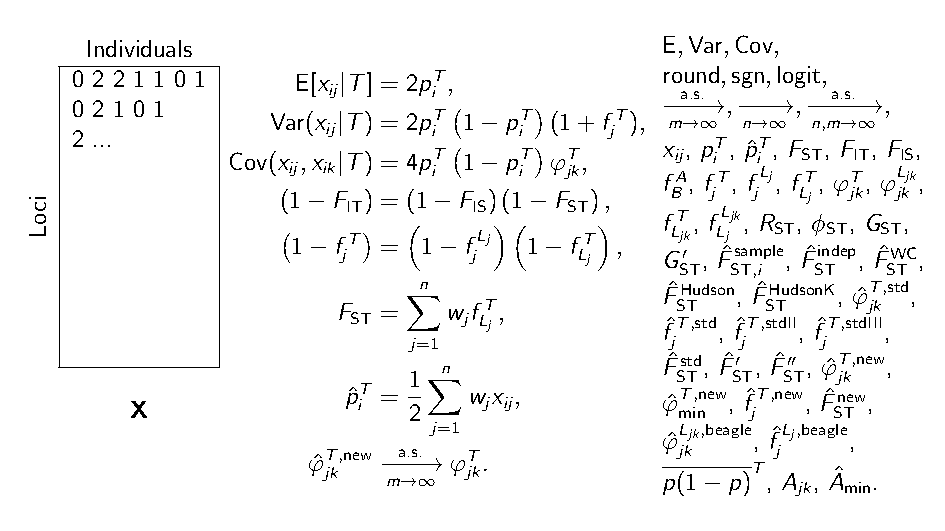
\includegraphics[width=\textwidth]{examples/test-vanilla.pdf}%
% \caption{The vanilla version of the symbols (no colors and no omission of ancestral population $T$ in superscripts}%
% \label{fig:vanilla}%
% \end{center}%
% \end{figure}%
% 
% \begin{figure}%
% \begin{center}%
% 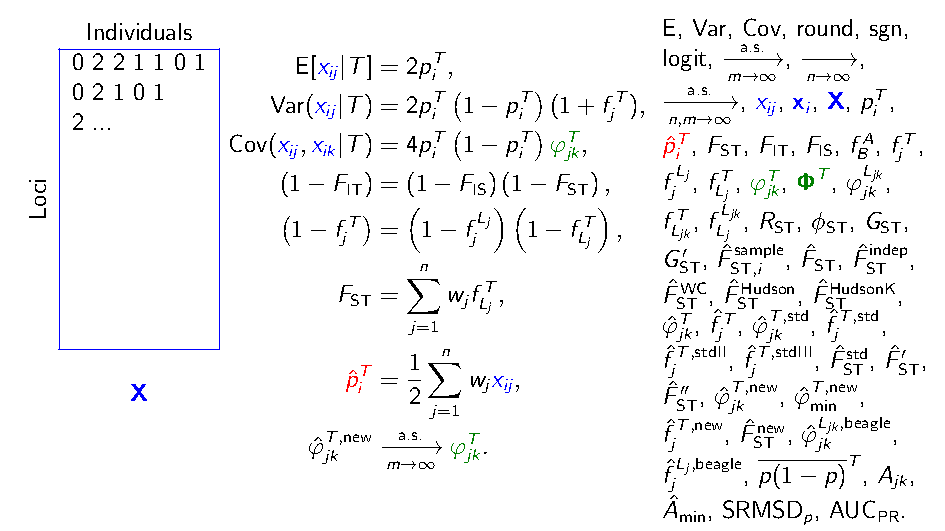
\includegraphics[width=\textwidth]{examples/test-color.pdf}%
% \caption{The \texttt{color} version of the symbols (with no omission of ancestral population $T$ in superscripts}%
% \label{fig:color}%
% \end{center}%
% \end{figure}%
% 
% \begin{figure}%
% \begin{center}%
% 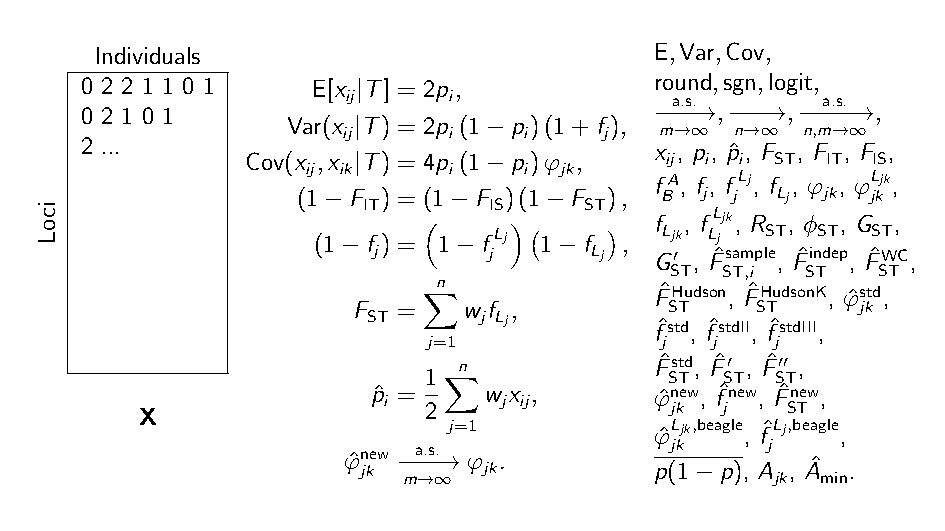
\includegraphics[width=\textwidth]{examples/test-noT.pdf}%
% \caption{The \texttt{noT} version of the symbols (no color, with omission of ancestral population $T$ in superscripts as appropriate}%
% \label{fig:noT}%
% \end{center}%
% \end{figure}%
% 
% \begin{figure}%
% \begin{center}%
% 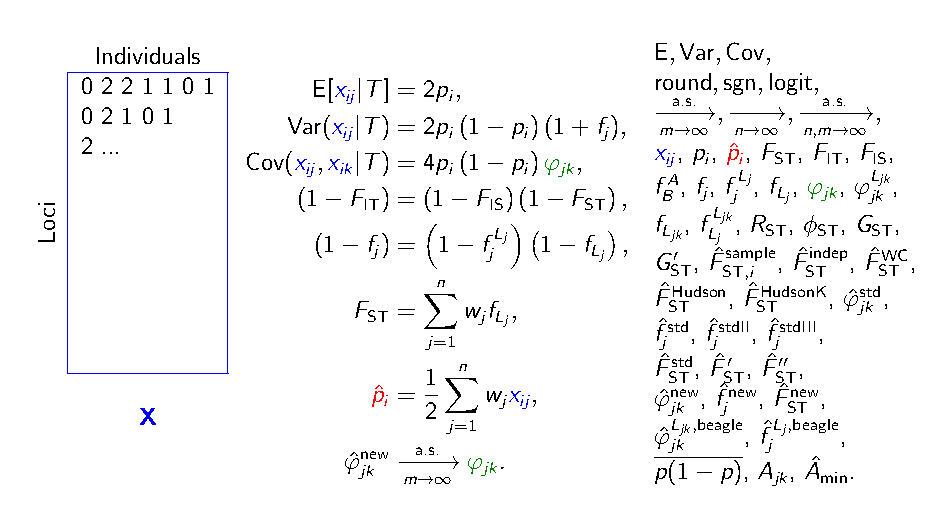
\includegraphics[width=\textwidth]{examples/test-color-noT.pdf}%
% \caption{The \texttt{color,noT} version of the symbols (with color and omission of ancestral population $T$ in superscripts as appropriate}%
% \label{fig:colorNoT}%
% \end{center}%
% \end{figure}%
% 
%
% \StopEventually{\PrintChanges\PrintIndex}
%
% \section{Implementation}
%
% \subsection{Dependencies}
% 
% This package requires
% |amsmath| to define the various math symbols and operators,
% |xspace| to allow inline math symbols to have appropriate spacings when used outside math mode,
% |xcolor| for color management and tricks, and
% |colortbl| and |multirow| for the cartoon genotype matrix.
%    \begin{macrocode}
\RequirePackage{amsmath}
\RequirePackage{xspace}
\RequirePackage{xcolor}
\RequirePackage{colortbl}
\RequirePackage{multirow}
%    \end{macrocode}
%
% \subsection{Initializing variables, modify depending on options}
% 
% Then we define the special colors we want to use (in a way that is easy to tweak later if needed).
% 
% \begin{macro}{\ifcolor}
%   LaTeX boolean for whether color option is on or off.
%    \begin{macrocode}
\newif\ifcolor%
\colorfalse% default is false
%    \end{macrocode}
% \end{macro}
% 
% \begin{macro}{genColor}
%   The hardcoded ``genotype color'' is blue, applied if the |color| package option is set.
%    \begin{macrocode}
\colorlet{genColor}{blue}
%    \end{macrocode}
% \end{macro}
% 
% \begin{macro}{kinColor}
%   The hardcoded ``kinship color'' is a dark green, applied if the |color| package option is set.
%    \begin{macrocode}
\colorlet{kinColor}{green!50!black}
%    \end{macrocode}
% \end{macro}
% 
% \begin{macro}{pithColor}
%   The hardcoded ``|\pith| color'' is red, applied if the |color| package option is set.
%    \begin{macrocode}
\colorlet{pithColor}{red}
%    \end{macrocode}
% \end{macro}
% 
% We also define two tricky commands to handle the ancestra population $T$ superscript that we want to optionally omit.
% Note that these are internal commands not meant to be used directly outside the package.
% 
% \begin{macro}{\kinshipsymbols@T}
%   This is a basic superscript $T$ that becomes blank if the |noT| package option is set.
%    \begin{macrocode}
\newcommand{\kinshipsymbols@T}{^T}
%    \end{macrocode}
% \end{macro}
% 
% \begin{macro}{\kinshipsymbols@Ts}
%   This is a second superscript $T$ which takes a mandatory argument that is shown next to it as text.
%   Only the $T$ becomes blank if the |noT| package option is set (the argument is shown alone as a text superscript in that case).
%    \begin{macrocode}
\newcommand{\kinshipsymbols@Ts}[1]{^{T,\text{#1}}}
%    \end{macrocode}
% \end{macro}
% 
% This turns on colors if the |color| package option is set.
%    \begin{macrocode}
\DeclareOption{color}{
  \colortrue
}
%    \end{macrocode}
% 
% Similarly, this updates the commands to omit the $T$ superscript if the |noT| package option is set.
% Note that the second command still emits the additional text passed as argument in the superscript.
%    \begin{macrocode}
\DeclareOption{noT}{
  \renewcommand{\kinshipsymbols@T}{}
  \renewcommand{\kinshipsymbols@Ts}[1]{^{\text{#1}}}
}
%    \end{macrocode}
% 
% This creates a warning if any additional options are passed, then processes the options.
%    \begin{macrocode}
\DeclareOption*{\PackageWarning{examplepackage}{Unknown ‘\CurrentOption’}}
\ProcessOptions\relax
%    \end{macrocode}
%
% \subsection{Commands for math operators}
%
%   Here we define some trivial widely-used operators, which are not specific to statistical genetics but which are absent from the standard |amsmath| package.
% 
% \begin{macro}{\E}
%   Expectation of a random variable.
%    \begin{macrocode}
\DeclareMathOperator{\E}{E}
%    \end{macrocode}
% \end{macro}
% 
% \begin{macro}{\Var}
%   Variance of a random variable.
%    \begin{macrocode}
\DeclareMathOperator{\Var}{Var}
%    \end{macrocode}
% \end{macro}
% 
% \begin{macro}{\Cov}
%   Covariance of a random variable.
%    \begin{macrocode}
\DeclareMathOperator{\Cov}{Cov}
%    \end{macrocode}
% \end{macro}
% 
% \begin{macro}{\round}
%   The rounding function.
%    \begin{macrocode}
\DeclareMathOperator{\round}{round}
%    \end{macrocode}
% \end{macro}
% 
% \begin{macro}{\sgn}
%   The sign function.
%    \begin{macrocode}
\DeclareMathOperator{\sgn}{sgn}
%    \end{macrocode}
% \end{macro}
% 
% \begin{macro}{\logit}
%   The logit function.
%    \begin{macrocode}
\DeclareMathOperator{\logit}{logit}
%    \end{macrocode}
% \end{macro}
%
% \subsection{Genotypes}
%
% \begin{macro}{\xij}
%   \xij:
%   Genotype variable at locus $i$ of individual $j$ (default).
%   The optional argument allows setting other individuals (|\xij[k]| gives \xij[k] for individual $k$).
%   If the package option |color| is passed, then this symbol turns the color |genColor| (default blue).
%    \begin{macrocode}
\newcommand{\xij}[1][j]{%
  \ensuremath{%
    \ifcolor \textcolor{genColor}{ \fi%
      x_{i#1}%
    \ifcolor } \fi%
  }%
  \xspace%
}%
%    \end{macrocode}
% \end{macro}
% 
% \subsection{Ancestral allele frequencies}
%
% \begin{macro}{\pit}
%   \pit:
%   The ancestral allele frequency at locus $i$.
%   This parameter has a value that depends on the ancestral population $T$, which is by default denoted in the superscript, but which gets omitted if the package option |noT| is passed.
%    \begin{macrocode}
\newcommand{\pit}{%
  \ensuremath{%
    p_i\kinshipsymbols@T%
  }%
  \xspace%
}%
%    \end{macrocode}
% \end{macro}
%
% \begin{macro}{\pith}
%   \pith:
%   The sample estimator of the ancestral allele frequency at locus $i$.
%   The parameter being estimated has a value that depends on the ancestral population $T$, which is by default denoted in the superscript, but which gets omitted if the package option |noT| is passed.
%   If the package option |color| is passed, then this symbol turns the color |pithColor| (default red).
%    \begin{macrocode}
\newcommand{\pith}{%
  \ensuremath{%
    \ifcolor \textcolor{pithColor}{ \fi%
      \hat{p}_i\kinshipsymbols@T%
    \ifcolor } \fi%
  }%
  \xspace%
}%
%    \end{macrocode}
% \end{macro}
%
% \subsection{Wright's \Fst}
%
% \begin{macro}{\Fst}
%   \Fst:
%   Wright's Fixation index.
%   Although the $T$ in the subscript technically refers to the ancestral population $T$, in this case it is never omitted (even if the package option |noT| is passed) to always match the more traditional and highly recognizable notation.
%    \begin{macrocode}
\newcommand{\Fst}{%
  \ensuremath{%
    F_{\text{ST}}%
  }%
  \xspace%
}%
%    \end{macrocode}
% \end{macro}
%
% \begin{macro}{\Fit}
%   \Fit:
%   Wright's total inbreeding coefficient.
%   Although the $T$ in the subscript technically refers to the ancestral population $T$, in this case it is never omitted (even if the package option |noT| is passed) to always match the more traditional and highly recognizable notation.
%    \begin{macrocode}
\newcommand{\Fit}{%
  \ensuremath{%
    F_{\text{IT}}%
  }%
  \xspace%
}%
%    \end{macrocode}
% \end{macro}
%
% \begin{macro}{\Fis}
%   \Fis:
%   Wright's local inbreeding coefficient.
%    \begin{macrocode}
\newcommand{\Fis}{%
  \ensuremath{%
    F_{\text{IS}}%
  }%
  \xspace%
}%
%    \end{macrocode}
% \end{macro}
%
% \subsection{Inbreeding coefficients}
%
% \begin{macro}{\f}
%   \f{A}{B}:
%   The inbreeding coefficient (of \Fst) of population $B$ relative to an ancestral population $A$.
%   Note that this command has two mandatory arguments.
%    \begin{macrocode}
\newcommand{\f}[2]{%
  \ensuremath{%
    f^{#1}_{#2}%
  }%
  \xspace%
}%
%    \end{macrocode}
% \end{macro}
%
% \begin{macro}{\ft}
%   \ft:
%   The (total) inbreeding coefficient of individual $j$ (default).
%   The optional argument allows setting other individuals (|\ft[k]| gives \ft[k] for individual $k$).
%   This parameter has a value that depends on the ancestral population $T$, which is by default denoted in the superscript, but which gets omitted if the package option |noT| is passed.
%    \begin{macrocode}
\newcommand{\ft}[1][j]{%
  \ensuremath{%
    f_{#1}\kinshipsymbols@T%
  }%
  \xspace%
}%
%    \end{macrocode}
% \end{macro}
%
% \begin{macro}{\fl}
%   \fl:
%   The local inbreeding coefficient of individual $j$ (default).
%   The optional argument allows setting other individuals (|\fl[k]| gives \fl[k] for individual $k$).
%    \begin{macrocode}
\newcommand{\fl}[1][j]{%
  \ensuremath{%
    f_{#1}^{L_{#1}}%
  }%
  \xspace%
}%
%    \end{macrocode}
% \end{macro}
%
% \begin{macro}{\fs}
%   \fs:
%   The structural inbreeding coefficient of individual $j$ (default).
%   The optional argument allows setting other individuals (|\fs[k]| gives \fs[k] for individual $k$).
%   This parameter has a value that depends on the ancestral population $T$, which is by default denoted in the superscript, but which gets omitted if the package option |noT| is passed.
%    \begin{macrocode}
\newcommand{\fs}[1][j]{%
  \ensuremath{%
    f_{L_{#1}}\kinshipsymbols@T%
  }%
  \xspace%
}%
%    \end{macrocode}
% \end{macro}
%
% \subsection{Kinship coefficients}
%
% \begin{macro}{\kt}
%   \kt:
%   The (total) kinship coefficient between the pair of individuals $j$ and $k$ (default).
%   The optional argument allows setting another second individual (|\kt[l]| gives \kt[l] for a second individual $l$).
%   This parameter has a value that depends on the ancestral population $T$, which is by default denoted in the superscript, but which gets omitted if the package option |noT| is passed.
%   If the package option |color| is passed, then this symbol turns the color |kinColor| (default dark green).
%    \begin{macrocode}
\newcommand{\kt}[1][k]{%
  \ensuremath{%
    \ifcolor \textcolor{kinColor}{ \fi%
      \varphi_{j#1}\kinshipsymbols@T%
    \ifcolor } \fi%
  }%
  \xspace%
}%
%    \end{macrocode}
% \end{macro}
%
% \begin{macro}{\kl}
%   \kl:
%   The local kinship coefficient between the pair of individuals $j$ and $k$.
%    \begin{macrocode}
\newcommand{\kl}{%
  \ensuremath{%
    \varphi_{jk}^{L_{jk}}%
  }%
  \xspace%
}%
%    \end{macrocode}
% \end{macro}
%
% \begin{macro}{\ks}
%   \ks:
%   The structural kinship coefficient between the pair of individuals $j$ and $k$.
%   This parameter has a value that depends on the ancestral population $T$, which is by default denoted in the superscript, but which gets omitted if the package option |noT| is passed.
%    \begin{macrocode}
\newcommand{\ks}{%
  \ensuremath{%
    f_{L_{jk}}\kinshipsymbols@T%
  }%
  \xspace%
}%
%    \end{macrocode}
% \end{macro}
%
% \begin{macro}{\fpw}
%   \fpw:
%   A component of the pairwise \Fst between a pair of individuals $j$ and $k$ (default).
%   The optional argument changes the individual in the subscript only (so |\fpw[k]| gives \fpw[k], and is obviously intended to be used for $k$ only).
%   Note that the actual pairwise \Fst between $j$ and $k$ is given by the average of \fpw and \fpw[k].
%    \begin{macrocode}
\newcommand{\fpw}[1][j]{%
  \f{L_{jk}}{L_{#1}}%
}%
%    \end{macrocode}
% \end{macro}
%
% \subsection{Review of previous work}
%
% \begin{macro}{\Rst}
%   \Rst:
%   An \Fst estimator developed for microsatellites.
%    \begin{macrocode}
\newcommand{\Rst}{%
  \ensuremath{%
    R_{\text{ST}}%
  }%
  \xspace%
}%
%    \end{macrocode}
% \end{macro}
%
% \begin{macro}{\PhiSt}
%   \PhiSt:
%   An \Fst-like estimate based on AMOVA.
%    \begin{macrocode}
\newcommand{\PhiSt}{%
  \ensuremath{%
    \phi_{\text{ST}}%
  }%
  \xspace%
}%
%    \end{macrocode}
% \end{macro}
%
% \begin{macro}{\Gst}
%   \Gst:
%   Nei's genetic diversity measure.
%    \begin{macrocode}
\newcommand{\Gst}{%
  \ensuremath{%
    G_{\text{ST}}%
  }%
  \xspace%
}%
%    \end{macrocode}
% \end{macro}
%
% \begin{macro}{\GstPrime}
%   \GstPrime:
%   A normalized \Gst statistic.
%    \begin{macrocode}
\newcommand{\GstPrime}{%
  \ensuremath{%
    G_{\text{ST}}'%
  }%
  \xspace%
}%
%    \end{macrocode}
% \end{macro}
%
% \begin{macro}{\FstHatSample}
%   \FstHatSample:
%   A sample \Fst estimator for a single locus $i$.
%    \begin{macrocode}
\newcommand{\FstHatSample}{%
  \ensuremath{%
    \hat{F}_{\text{ST},i}^{\text{sample}}%
  }%
  \xspace%
}%
%    \end{macrocode}
% \end{macro}
%
% \subsection{Convergence arrows}
%
% \begin{macro}{\toas}
%   $\toas$:
%   Almost sure convergence as $m$ goes to $\infty$.
%    \begin{macrocode}
\newcommand{\toas}{%
  \xrightarrow[m \rightarrow \infty]{\text{a.s.}}
}%
%    \end{macrocode}
% \end{macro}
%
% \begin{macro}{\toN}
%   $\toN$:
%   The limit as $n$ goes to $\infty$.
%   Optional argument changes the variable name (|$\toN[m]$| gives $\toN[m]$).
%    \begin{macrocode}
\newcommand{\toN}[1][n]{%
  \xrightarrow[#1 \rightarrow \infty]{}%
}%
%    \end{macrocode}
% \end{macro}
%
% \begin{macro}{\toasNM}
%   $\toasNM$:
%   Almost sure convergence as both $n$ and $m$ go to $\infty$.
%    \begin{macrocode}
\newcommand{\toasNM}{%
  \xrightarrow[n,m \rightarrow \infty]{\text{a.s.}}%
}%
%    \end{macrocode}
% \end{macro}
%
% \subsection{\Fst estimators for independent subpopulations}
%
% \begin{macro}{\FstHatNamed}
%   \FstHatNamed{example}:
%   Base command for a named \Fst estimator.
%   Takes on one mandatory argument---the name of the estimator---which is rendered as text.
%    \begin{macrocode}
\newcommand{\FstHatNamed}[1]{%
  \ensuremath{%
    \hat{F}_{\text{ST}}^{\text{#1}}%
  }%
  \xspace%
}%
%    \end{macrocode}
% \end{macro}
%
% \begin{macro}{\FstHatIs}
%   \FstHatIs:
%   Asymptotic \Fst estimator for independent subpopulations.
%    \begin{macrocode}
\newcommand{\FstHatIs}{\FstHatNamed{indep}}
%    \end{macrocode}
% \end{macro}
%
% \begin{macro}{\FstHatWc}
%   \FstHatWc:
%   Weir-Cockerham \Fst estimator.
%    \begin{macrocode}
\newcommand{\FstHatWc}{\FstHatNamed{WC}}
%    \end{macrocode}
% \end{macro}
%
% \begin{macro}{\FstHatHudson}
%   \FstHatHudson:
%   Hudson pairwise \Fst estimator.
%    \begin{macrocode}
\newcommand{\FstHatHudson}{\FstHatNamed{Hudson}}
%    \end{macrocode}
% \end{macro}
%
% \begin{macro}{\FstHatHudsonK}
%   \FstHatHudsonK:
%   Generalized Hudson \Fst estimator (for $K$ subpopulations).
%    \begin{macrocode}
\newcommand{\FstHatHudsonK}{\FstHatNamed{HudsonK}}
%    \end{macrocode}
% \end{macro}
%
% \subsection{Estimators based on the standard kinship}
%
% \begin{macro}{\ktHatNamed}
%   \ktHatNamed{example}:
%   A generic named kinship estimator for individuals $j$ and $k$ (default).
%   Mandatory argument is the name, rendered as text.
%   The optional argument allows setting another second individual (|\ktHatNamed[l]{example}| gives \ktHatNamed[l]{example} for a second individual $l$).
%   The estimated parameter has a value that depends on the ancestral population $T$, which is by default denoted in the superscript, but which gets omitted if the package option |noT| is passed.
%    \begin{macrocode}
\newcommand{\ktHatNamed}[2][k]{%
  \ensuremath{%
    \hat{\varphi}_{j#1}\kinshipsymbols@Ts{#2}%
  }%
  \xspace%
}%
%    \end{macrocode}
% \end{macro}
%
% \begin{macro}{\ktHatStd}
%   \ktHatStd:
%   Standard kinship estimator for individuals $j$ and $k$ (default).
%   The optional argument allows setting another second individual (|\ktHatStd[l]| gives \ktHatStd[l] for a second individual $l$).
%   The estimated parameter has a value that depends on the ancestral population $T$, which is by default denoted in the superscript, but which gets omitted if the package option |noT| is passed.
%    \begin{macrocode}
\newcommand{\ktHatStd}[1][k]{\ktHatNamed[#1]{std}}
%    \end{macrocode}
% \end{macro}
%
% \begin{macro}{\ftHatNamed}
%   \ftHatNamed{example}:
%   Named inbreeding coefficient estimator for individual $j$ (default).
%   Mandatory argument is the name, rendered as text.
%   The optional argument allows setting another individual (|\ftHatNamed[k]{example}| gives \ftHatNamed[k]{example} for individual $k$).
%   The estimated parameter has a value that depends on the ancestral population $T$, which is by default denoted in the superscript, but which gets omitted if the package option |noT| is passed.
%    \begin{macrocode}
\newcommand{\ftHatNamed}[2][j]{%
  \ensuremath{%
    \hat{f}_{#1}\kinshipsymbols@Ts{#2}%
  }%
  \xspace%
}%
%    \end{macrocode}
% \end{macro}
%
% \begin{macro}{\ftHatStd}
%   \ftHatStd:
%   Standard inbreeding coefficient estimator (I) for individual $j$.
%   The estimated parameter has a value that depends on the ancestral population $T$, which is by default denoted in the superscript, but which gets omitted if the package option |noT| is passed.
%    \begin{macrocode}
\newcommand{\ftHatStd}{\ftHatNamed{std}}
%    \end{macrocode}
% \end{macro}
%
% \begin{macro}{\ftHatStdII}
%   \ftHatStdII:
%   Alternate inbreeding coefficient estimator (II) for individual $j$.
%   The estimated parameter has a value that depends on the ancestral population $T$, which is by default denoted in the superscript, but which gets omitted if the package option |noT| is passed.
%    \begin{macrocode}
\newcommand{\ftHatStdII}{\ftHatNamed{stdII}}
%    \end{macrocode}
% \end{macro}
%
% \begin{macro}{\ftHatStdIII}
%   \ftHatStdIII:
%   Alternate inbreeding coefficient estimator (III) for individual $j$.
%   The estimated parameter has a value that depends on the ancestral population $T$, which is by default denoted in the superscript, but which gets omitted if the package option |noT| is passed.
%    \begin{macrocode}
\newcommand{\ftHatStdIII}{\ftHatNamed{stdIII}}
%    \end{macrocode}
% \end{macro}
%
% \begin{macro}{\FstHatStd}
%   \FstHatStd:
%   Standard \Fst estimator (based on the standard kinship estimator).
%    \begin{macrocode}
\newcommand{\FstHatStd}{\FstHatNamed{std}}
%    \end{macrocode}
% \end{macro}
%
% \begin{macro}{\FstHatStdPrime}
%   \FstHatStdPrime:
%   Standard \Fst estimator adjusted 1.
%    \begin{macrocode}
\newcommand{\FstHatStdPrime}{%
  \ensuremath{%
    \hat{F}_{\text{ST}}'%
  }%
  \xspace%
}%
%    \end{macrocode}
% \end{macro}
%
% \begin{macro}{\FstHatStdPrimeDbl}
%   \FstHatStdPrimeDbl:
%   Standard \Fst estimator adjusted 2.
%    \begin{macrocode}
\newcommand{\FstHatStdPrimeDbl}{%
  \ensuremath{%
    \hat{F}_{\text{ST}}''%
  }%
  \xspace%
}%
%    \end{macrocode}
% \end{macro}
%
% \subsection{New kinship and \Fst estimators}
%
% \begin{macro}{\ktHatNew}
%   \ktHatNew:
%   New kinship estimator for the pair of individuals $j$ and $k$ (default).
%   The optional argument allows setting another second individual (|\ktHatNew[l]| gives \ktHatNew[l] for a second individual $l$).
%   The estimated parameter has a value that depends on the ancestral population $T$, which is by default denoted in the superscript, but which gets omitted if the package option |noT| is passed.
%    \begin{macrocode}
\newcommand{\ktHatNew}[1][k]{\ktHatNamed[#1]{new}}
%    \end{macrocode}
% \end{macro}
%
% \begin{macro}{\ftHatNew}
%   \ftHatNew:
%   New inbreeding estimator for individual $j$ (default).
%   The optional argument allows setting other individuals (|\ftHatNew[k]| gives \ftHatNew[k] for individual $k$).
%   The estimated parameter has a value that depends on the ancestral population $T$, which is by default denoted in the superscript, but which gets omitted if the package option |noT| is passed.
%    \begin{macrocode}
\newcommand{\ftHatNew}[1][j]{\ftHatNamed[#1]{new}}
%    \end{macrocode}
% \end{macro}
%
% \begin{macro}{\FstHatNew}
%   \FstHatNew:
%   New \Fst estimator.
%    \begin{macrocode}
\newcommand{\FstHatNew}{\FstHatNamed{new}}
%    \end{macrocode}
% \end{macro}
%
% \begin{macro}{\Ajk}
%   \Ajk:
%   A new statistic proportional in expectation to $\kt-1$ for the pair of individuals $j$ and $k$ (default).
%   The optional argument allows setting another second individual (|\Ajk[l]| gives \Ajk[l] for a second individual $l$).
%    \begin{macrocode}
\newcommand{\Ajk}[1][k]{%
  \ensuremath{%
    A_{j#1}%
  }%
  \xspace%
}%
%    \end{macrocode}
% \end{macro}
%
% \begin{macro}{\AMinHat}
%   \AMinHat:
%   Estimator of the limit of the minimum value of the expectation of \Ajk across all pairs of individuals.
%    \begin{macrocode}
\newcommand{\AMinHat}{%
  \ensuremath{%
    \hat{A}_{\text{min}}%
  }%
  \xspace%
}%
%    \end{macrocode}
% \end{macro}
%
% \begin{macro}{\AAvgHat}
%   \AAvgHat:
%   Estimator of the limit of the average value of the expectation of \Ajk across all pairs of individuals.
%    \begin{macrocode}
\newcommand{\AAvgHat}{%
  \ensuremath{%
    \hat{A}_{\text{avg}}%
  }%
  \xspace%
}%
%    \end{macrocode}
% \end{macro}
%
% \begin{macro}{\mav}
%   \mav:
%   Mean ancestral variance.
%   This parameter has a value that depends on the ancestral population $T$, which is by default denoted in the superscript, but which gets omitted if the package option |noT| is passed.
%    \begin{macrocode}
\newcommand{\mav}{%
  \ensuremath{%
    \overline{p(1-p)}\kinshipsymbols@T%
  }%
  \xspace%
}%
%    \end{macrocode}
% \end{macro}
%
% \subsection{Estimates from Beagle}
%
% \begin{macro}{\klHatBeagle}
%   \klHatBeagle:
%   Local kinship estimator based on Beagle, for the pair of individuals $j$ and $k$.
%    \begin{macrocode}
\newcommand{\klHatBeagle}{%
  \ensuremath{%
    \hat{\varphi}_{jk}^{L_{jk},\text{beagle}}%
  }%
  \xspace%
}%
%    \end{macrocode}
% \end{macro}
%
% \begin{macro}{\flHatBeagle}
%   \flHatBeagle:
%   Local inbreeding estimator based on Beagle, for individual $j$ (default).
%   The optional argument allows setting other individuals (|\flHatBeagle[k]| gives \flHatBeagle[k] for individual $k$).
%    \begin{macrocode}
\newcommand{\flHatBeagle}[1][j]{%
  \ensuremath{%
    \hat{f}_{#1}^{L_{#1},\text{beagle}}%
  }%
  \xspace%
}%
%    \end{macrocode}
% \end{macro}
%
% \subsection{Cartoon genotype matrix}
%
% I use this cartoon genotype matrix often in Beamer presentations.
% Unfortunately I also use the |color| kinshipsymbols package option in my presentations, but due to a strange bug the colors do not show up in Beamer.
% This solution was found online:
% \url{https://tex.stackexchange.com/questions/159378/cline-disappears-in-beamer}
%    \begin{macrocode}
% after package colortbl is loaded
\makeatletter
\@ifclassloaded{beamer}{%
  \patchcmd\@cline
      {\arrayrulewidth\hfill}% search
      {\arrayrulewidth\hfill\kern\z@}% replace
      {}% success
      {\errmessage{Patching \string\@cline\space failed}}% failure
}{%
  % nothing to do here?
}
\makeatother
%    \end{macrocode}
%
% \begin{macro}{\sampleGenMat}
%   This is the bulky code used to generate the cartoon genotype matrix shown in \cref{fig:sampleGenMat}.
%    \begin{macrocode}
\newcommand{\sampleGenMat}{%
  \begin{tabular}{cc}%
    & Individuals \\%
    \ifcolor \arrayrulecolor{genColor} \fi% % gets applied to whole table
    \cline{2-2}%
    \multirow{10}{*}{\rotatebox[origin=c]{90}{Loci}}%
    & \multicolumn{1}{|l|}{0 2 2 1 1 0 1} \\%
    & \multicolumn{1}{|l|}{0 2 1 0 1 } \\%
    & \multicolumn{1}{|l|}{2 ...} \\%
    & \multicolumn{1}{|l|}{ } \\%
    & \multicolumn{1}{|l|}{ } \\%
    & \multicolumn{1}{|l|}{ } \\%
    & \multicolumn{1}{|l|}{ } \\%
    & \multicolumn{1}{|l|}{ } \\%
    & \multicolumn{1}{|l|}{ } \\%
    & \multicolumn{1}{|l|}{ } \\%
    \cline{2-2}%
    & \\%
    & $\mathbf{
      \ifcolor \textcolor{genColor}{ \fi%
      X
      \ifcolor } \fi%
      }$ \\%
  \end{tabular}%
}%
%    \end{macrocode}
% \end{macro}
%
% \section{Acknowledgments}
%
% The symbols in this package were originally designed with John D. Storey (Alex Ochoa's postdoctoral adviser and coauthor of several papers about kinship and \Fst).
% 
% The package was written following Scott Pakin's guide
% \href{http://texdoc.net/texmf-dist/doc/latex/dtxtut/dtxtut.pdf}{How to Package Your \LaTeX~package}.
%
% \Finale
\endinput
